\subsection{Assessing porosity}

Characterization of the pore size and their distribution in porous materials
is often the main goal when performing adsorption experiments. It is 
therefore important that pyGAPS includes several robust methods 
for determining pore distribution from isotherm data.

When it comes to porous materials, three kinds of pore sizes have been
defined, based on their lengthscales: micropores (\SI{< 2}{\nano\metre}),
mesopores (\SIrange{2}{50}{\nano\metre}), and macropores (\SI{> 50}{\nano\metre}).

Macropores are generally unable to be characterised through adsorption, with 
methods such as mercury intrusion porosimetry as the standard for pore
size distributions in this lengthscale, although other alternatives have 
been suggested~\cite{rouquerolCharacterizationMacroporousSolids2012} due
to the high toxicity of mercury. Therefore, they are outside the scope
of this framework.

In the mesopore range, the \textit{``classical''} methods are usually applied,
based on the application of Kelvin's equation pertaining to capillary 
condensation. This equation calculates the critical pressure at which 
the fluid completely files a pore of a specific length. This equation,
applicable to a range of geometries, is used in multiple approaches
such as the original Barrett-Joyner-Halenda (BJH) method or the 
Dollimore-Heal (DH) method.

For microporous materials, the Kelvin equation with its assumptions 
of continuous fluid properties and equal density of the adsorbed 
state to bulk liquid density breaks down. An atomistic approach
is required here, to address the interaction between solid-fluid
and fluid-fluid through potential functions. The Horvath-Kawazoe or 
HK method is often used, and it is implemented in pyGAPS.

Finally, methods based on density functional theory (DFT) and similar
variants such as non-local DFT (NLDFT) and quenched solid state DFT
(QSDFT) should be mentioned, as they can be used for multiscale
(micropore and mesopore) characterisation. These methods rely on the
\textit{in-silico} simulation of isotherms on a range of pore sizes,
which can then be collated in a so-called \textit{kernel} able to
be used in decomposition of a experimental isotherm to obtain a 
pore size distribution. While the generation of DFT kernels is 
outside the scope of the pyGAPS framework, it is able to use 
user-provided kernels to fit adsorption isotherms, and comes with 
a basic kernel for \ce{N2} adsorption at \SI{77}{\kelvin} on carbon slit pores.

It should be noted that all methods described require knowledge of
the pore geometry as well as depend on the material having pores which
conform to this well-defined shape. Real adsorbents usually have interconnected
networks of irregular pores, which may only be approximated by the
ideal pores used in these models.


\subsubsection{Mesoporous size distribution}

\paragraph{The Kelvin equation}

Since the Kelvin equation is the basis of both the BJH and DH methods
its theory and its implementation will be described here.



According to Rouquerol~\cite{rouquerolAdsorptionPowdersPorous2013}, 
in adopting this approach, it is assumed that:

\begin{itemize}
    
    \item The Kelvin equation is applicable over the pore range (mesopores). Therefore
    in pores which are below a certain size (around 2.5 nm), the granularity
    of the liquid-vapour interface becomes too large for classical bulk methods
    to be applied.
    \item The meniscus curvature is controlled be the pore size and shape. Ideal shapes
    for the curvature are assumed.
    \item The pores are rigid and of well defined shape. They are considered
    open-ended and non-intersecting
    \item The filling/emptying of each pore does not depend on its location.
    \item The adsorption on the pore walls is not different from surface adsorption.
        
\end{itemize}


The Kelvin equation assumes that adsorption in a pore is not different than adsorption
on a standard surface. Therefore, no interactions with the adsorbent is accounted for.
Furthermore, the geometry of the pore itself is considered to be invariant across the
entire adsorbate.

\paragraph{Barrett, Joyner and Halenda (BJH) pore size distribution}


Calculates the pore size distribution using a \textit{classical} model which attempts to
describe the adsorption in a pore as a combination of a statistical thickness and
a condensation/evaporation behaviour described by surface tension

The BJH method for calculating pore size distribution
is based on a classical description of the adsorbate behaviour in the adsorbent
pores~\cite{barrettDeterminationPoreVolume1951}.
Under this method, the adsorbate is adsorbing on the pore walls in a predictable way,
and decreasing the apparent pore volume until condensation takes place, filling the
entire pore. The critical radius is a sum of two radii, the adsorbed 
layer thickness, which can be modelled by a thickness model
(such as Halsey, Harkins \& Jura as presented in Section~\ref{pyg:charac:tcurve}) 
and a critical radius model for condensation/evaporation, 
based on a form of the Kelvin equation.

\begin{equation}
    r_p = t + r_k
\end{equation}

The original model used the desorption curve as a basis for calculating pore size distribution.
Between two points of the curve, the volume desorbed can be described as the volume contribution
from pore evaporation and the volume from layer thickness decrease as per the equation
above. The computation is done cumulatively, starting from the filled pores and 
calculating for each point the volume adsorbed in a pore from the following equation:

\begin{align}
    V_p & = \Big( \frac{\bar{r}_p}{\bar{r}_k + \Delta t_n} \Big)^2
    \Big(\Delta V_n - \Delta t_n \sum_{i=1}^{n-1} \Delta A_p
    + \Delta t_n \bar{t}_n \sum_{i=1}^{n-1} \frac{\Delta A_p}{\bar{r}_p}\Big) \\
    A & = 2 \Delta V_p / r_p
\end{align}

Where:

\begin{itemize}
    
    \item \(\Delta A_p\) is the area of the pores
    \item \(\Delta V_p\) is the adsorbed volume change between two points
    \item \(\bar{r}_p\) is the average pore radius calculated as a sum of the
    kelvin radius and layer thickness of the pores at pressure p between two
    measurement points
    \item \(\bar{r}_k\) is the average kelvin radius between two measurement points
    \item \(\bar{t}_n\) is the average layer thickness between two measurement points
    \item \(\Delta t_n\) is the average change in layer thickness between two measurement points
    
\end{itemize}

Then, by plotting \(\Delta V / (2*\Delta r_p)\) versus the width of the pores calculated
for each point, the pore size distribution can be obtained.

\paragraph{Dollimore-Heal pore size distribution}

The DH or Dollimore-Heal method~\cite{dollimorePoresizeDistributionTypical1970} 
of calculation of pore size distribution is an
extension of the BJH method, which takes into account the geometry of the pores
by introducing a length component.

Like the BJH method, it is based on a classical description of the adsorbate behaviour
in the adsorbent pores. 

\begin{align}
    V_p & = \Big(\frac{\bar{r}_p}{\bar{r}_k + \Delta t_n}\Big)^2
    \Big(\Delta V_n - \Delta t_n \sum_{i=1}^{n-1} \Delta A_p
    + 2 \pi \Delta t_n \bar{t}_n \sum_{i=1}^{n-1} L_p\Big) \\
%
    A & = 2 \Delta V_p / r_p \\
%
    L & = \Delta A_p / 2 \pi r_p
\end{align}

Where:
\begin{itemize}
    
    \item \(\Delta A_p\) is the area of the pores
    \item \(\Delta V_p\) is the adsorbed volume change between two points
    \item \(\bar{r}_p\) is the average pore radius calculated as a sum of the
    kelvin radius and layer thickness of the pores at pressure p between two
    measurement points
    \item \(\bar{r}_k\) is the average kelvin radius between two measurement points
    \item \(\bar{t}_n\) is the average layer thickness between two measurement points
    \item \(\Delta t_n\) is the average change in layer thickness between two measurement points
\end{itemize}

Then, by plotting \(\Delta V/(2*\Delta r_p)\) versus the width of the pores calculated
for each point, the pore size distribution can be obtained.

\subsubsection{Microporous size distribution}

The H-K method attempts to describe the adsorption within pores by calculation
of the average potential energy for a pore~\cite{horvathMethodCalculationEffective1983}.
The method starts by assuming the
relationship between the gas phase as being:

\begin{equation}
    R_g T \ln(\frac{p}{p_0}) = U_0 + P_a
\end{equation}

Here \(U_0\) is the potential function describing the surface to adsorbent
interactions and \(P_a\) is the potential function describing the adsorbate-
adsorbate interactions. This equation is derived from the equation of the free energy
of adsorption at constant temperature where term \(T \Delta S^{tr}(w/w_{\infty})\)
is assumed to be negligible.

If a Lennard-Jones-type potential function describes the interactions between the
adsorbate molecules and the adsorbent molecules then the two contributions to the
total potential can be replaced by the extended function. The resulting equation becomes

\begin{multline}
    RTln(p/p_0) =   N_A\frac{n_a A_a + n_A A_A}{2 \sigma^{4}(l-d)} \\
                    \times \int_{d/_2}^{1-d/_2}
                        \Big[
                        - \Big(\frac{\sigma}{r}\Big)^{4}
                        + \Big(\frac{\sigma}{r}\Big)^{10}
                        - \Big(\frac{\sigma}{l-r}\Big)^{4}
                        + \Big(\frac{\sigma}{l-r}\Big)^{4}
                        \Big] \mathrm{d}x
\end{multline}

where \(l\) is the width of the pore, \(d\) defined as \(d=d_a+d_A\) is 
the sum of the diameters of the adsorbate and adsorbent molecules,
\(n_a\) is number of molecules of adsorbent
and \(A_a\) and \(A_A\) the Lennard-Jones potential constant of the
fluid molecule and solid molecule respectively which are defined as

\begin{align}
    A_a &= \frac{6mc^2\alpha_a\alpha_A}{\alpha_a/\varkappa_a + \alpha_A/\varkappa_A}
%
    \intertext{and}
%
    A_a &= \frac{3mc^2\alpha_A\varkappa_A}{2}
\end{align}

Here \(m\) is the mass of an electron, \(\alpha_a\) and \(\alpha_A\) are
the polarizability of the adsorbate and adsorbate molecule and \(\varkappa_a\)
and \(\varkappa_A\) the magnetic susceptibility of the adsorbate molecule
and adsorbent molecule, respectively.

The HK method is applicable to slit pores, and it can be modified to 
be extended to cylindrical and spherical pores. It is worth noting
that there are several assumptions made which limit its applicability:

\begin{itemize}
    
    \item It does not have a description of capillary condensation. This means that the
    pore size distribution can only be considered accurate up to a maximum of 5 nm.
    \item Each pore is modelled as uniform and of infinite length. Materials with varying pore
    shapes or highly interconnected networks may not give realistic results.
    \item The HK method is reliant on knowledge of the properties of the surface atoms.
    This assumption is true only if the material surface is homogenous. Furthermore,
    longer range interactions with multiple surface layers are not considered.
    \item Only dispersive forces are accounted for. If the adsorbate-adsorbent interactions
    have other specific contributions, the Lennard-Jones potential function will not be
    an accurate description of pore environment.
    
\end{itemize}

The pyGAPS framework contains the required physical properties for the most commonly
used adsorbates, as well as properties from literature for several materials: 
the original parameters developed by Horvath and Kawazoe for a carbon surface
~\cite{horvathMethodCalculationEffective1983} and the oxide surface parameters
published by Saito and Foley~\cite{saitoCurvatureParametricSensitivity1991}.
The user can provide custom dictionary of these parameters when calling the 
function. 

\begin{lstlisting}[caption={Using the HK method for PSD},label={pyg:lst:hkpsd}]
# Calling the HK micropore method with the 
# Saito-Foley oxide surface parameters
result_dict = pygaps.micropore_size_distribution(
    isotherm,
    psd_model='HK',
    adsorbent_model='OxideIon(SF)',
    verbose=True
)
# Defining a custom adsorbate parameter dictionary 
# and using it in the HK method
adsorbate_params = {
    'magnetic_susceptibility': 3.6e-35,
    'molecular_diameter': 0.3,
    'polarizability': 1.76e-30,
    'surface_density': 6.71e+18
}
result_dict = pygaps.micropore_size_distribution(
    isotherm,
    psd_model='HK',
    adsorbent_model='OxideIon(SF)',
    adsorbate_model=adsorbate_params,
    verbose=True
)

\end{lstlisting}

\begin{figure}[h!]
    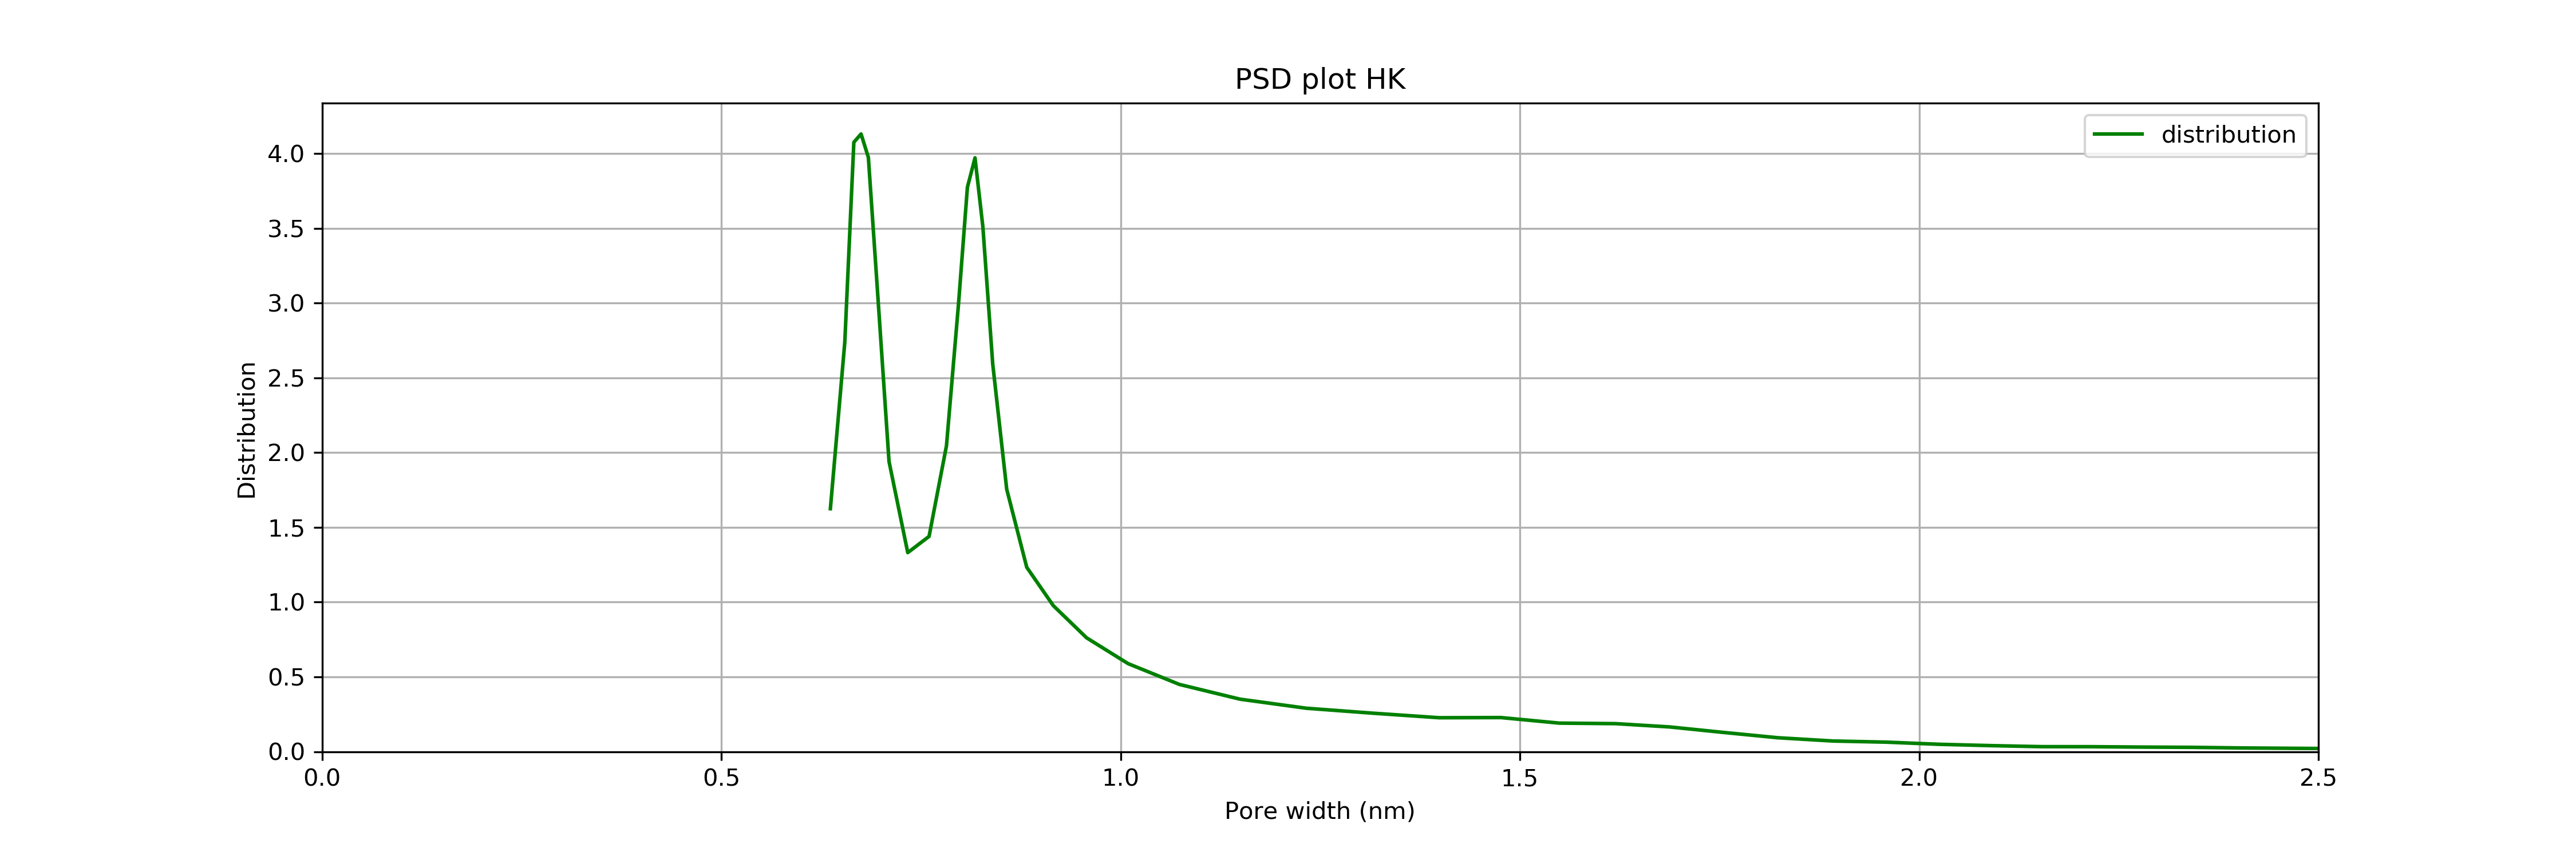
\includegraphics[width=\textwidth]{psd/hk}
    \caption{Pore size distribution calculated through the Horvath-Kawazoe method}%
    \label{fig:pyg:fig:hk}
\end{figure}

\subsubsection{DFT kernel fitting}

The function will take the data in the form of pressure and loading. It will
then load the kernel either from disk or from memory and define a minimization
function as the sum of squared differences of the sum of all individual kernel
isotherm loadings multiplied by their contribution as per the following function:

\begin{equation}
    f(x) = \sum_{p=p_0}^{p=p_x} (n_{p,exp} - \sum_{w=w_0}^{w=w_y} n_{p, kernel} X_w )^2
\end{equation}